\documentclass{article}
\usepackage{amsmath}
\usepackage{graphicx} % Add this line
\usepackage{xcolor}
\pagecolor{black}
\color{white}

\title{Rugsafe: A Protocol for Protecting Digital Assets from Rug Pulls}
\author{info@rugsafe.org}
\date{v0.0.1 August 1, 2024}

\begin{document}

\maketitle

\begin{abstract}
Rugsafe introduces a novel protocol designed to mitigate the risks associated with rug pulls in decentralized finance (DeFi). By leveraging cryptographic primitives and economic incentives, Rugsafe provides a framework that ensures the security and recoverability of assets when fraudulent activities are detected. The protocol is built around the concept of vaults for rugged tokens, issuance of anticoin tokens, and an incentive mechanism that penalizes and rewards users based on their interaction with the system. Rugsafe integrates seamlessly with existing DeFi platforms, offering an additional layer of security without compromising the decentralization principles.
\end{abstract}

%\clearpage

%\tableofcontents

%\twocolumn
\section{Overview}

The Rugsafe protocol enables users who hold rugged tokens, denoted as $C_r$, to deposit these tokens into a specialized vault $V_c$ and receive an equal amount of anticoin tokens, $C_a$, which are pegged to the inverse price movement of $C_r$.


%%%%%%%%%%%%%%%%%%%%%%


\subsection{Vault Creation and Anticoin Issuance}
When a vault $V_c$ is created for a rugged token $C_r$, users can deposit $C_r$ into this vault. Upon deposit, the protocol mints an equal amount of $C_a$, which is credited to the user's balance.

\begin{equation}
C_a = C_r
\end{equation}

The vaults are held in a central vault registry, ensuring that all interactions with rugged tokens are tracked and managed within the system.


%%%%%%%%%%%%%%%%%%%%%%%%%%%%%


\subsection{Withdrawal Penalty Mechanism}
If a user decides to withdraw their original rugged tokens $C_r$ by depositing back their $C_a$, a penalty is incurred. A portion of the $C_a$ tokens are deducted from the user's balance, and these penalized tokens are distributed among the remaining $C_a$ holders.

\begin{equation}
C_{r,\text{withdrawn}} = C_{r,\text{deposited}} - P(C_a)
\end{equation}

Where $P(C_a)$ represents the penalty, which scales according to the amount of $C_r$ originally deposited. The penalty mechanism incentivizes holding $C_a$ longer, as the remaining holders benefit from these penalties.




%%%%%%%%%%%%%%%%%%%%%%%%%%%%






\subsection{Anticoin Pricing and Pegging Mechanism}
At the time of vault creation, the protocol records the current price of the underlying rugged token $C_r$. This price is used as a reference for all future transactions involving $C_a$.

\begin{equation}
\text{Price}_{C_a} \propto \frac{1}{\text{Price}_{C_r}}
\end{equation}

As the price of $C_r$ fluctuates, the value of $C_a$ adjusts inversely, similar to an algorithmic stablecoin mechanism. This ensures that $C_a$ holders are protected against the devaluation of $C_r$.

\begin{figure}[h]
\centering
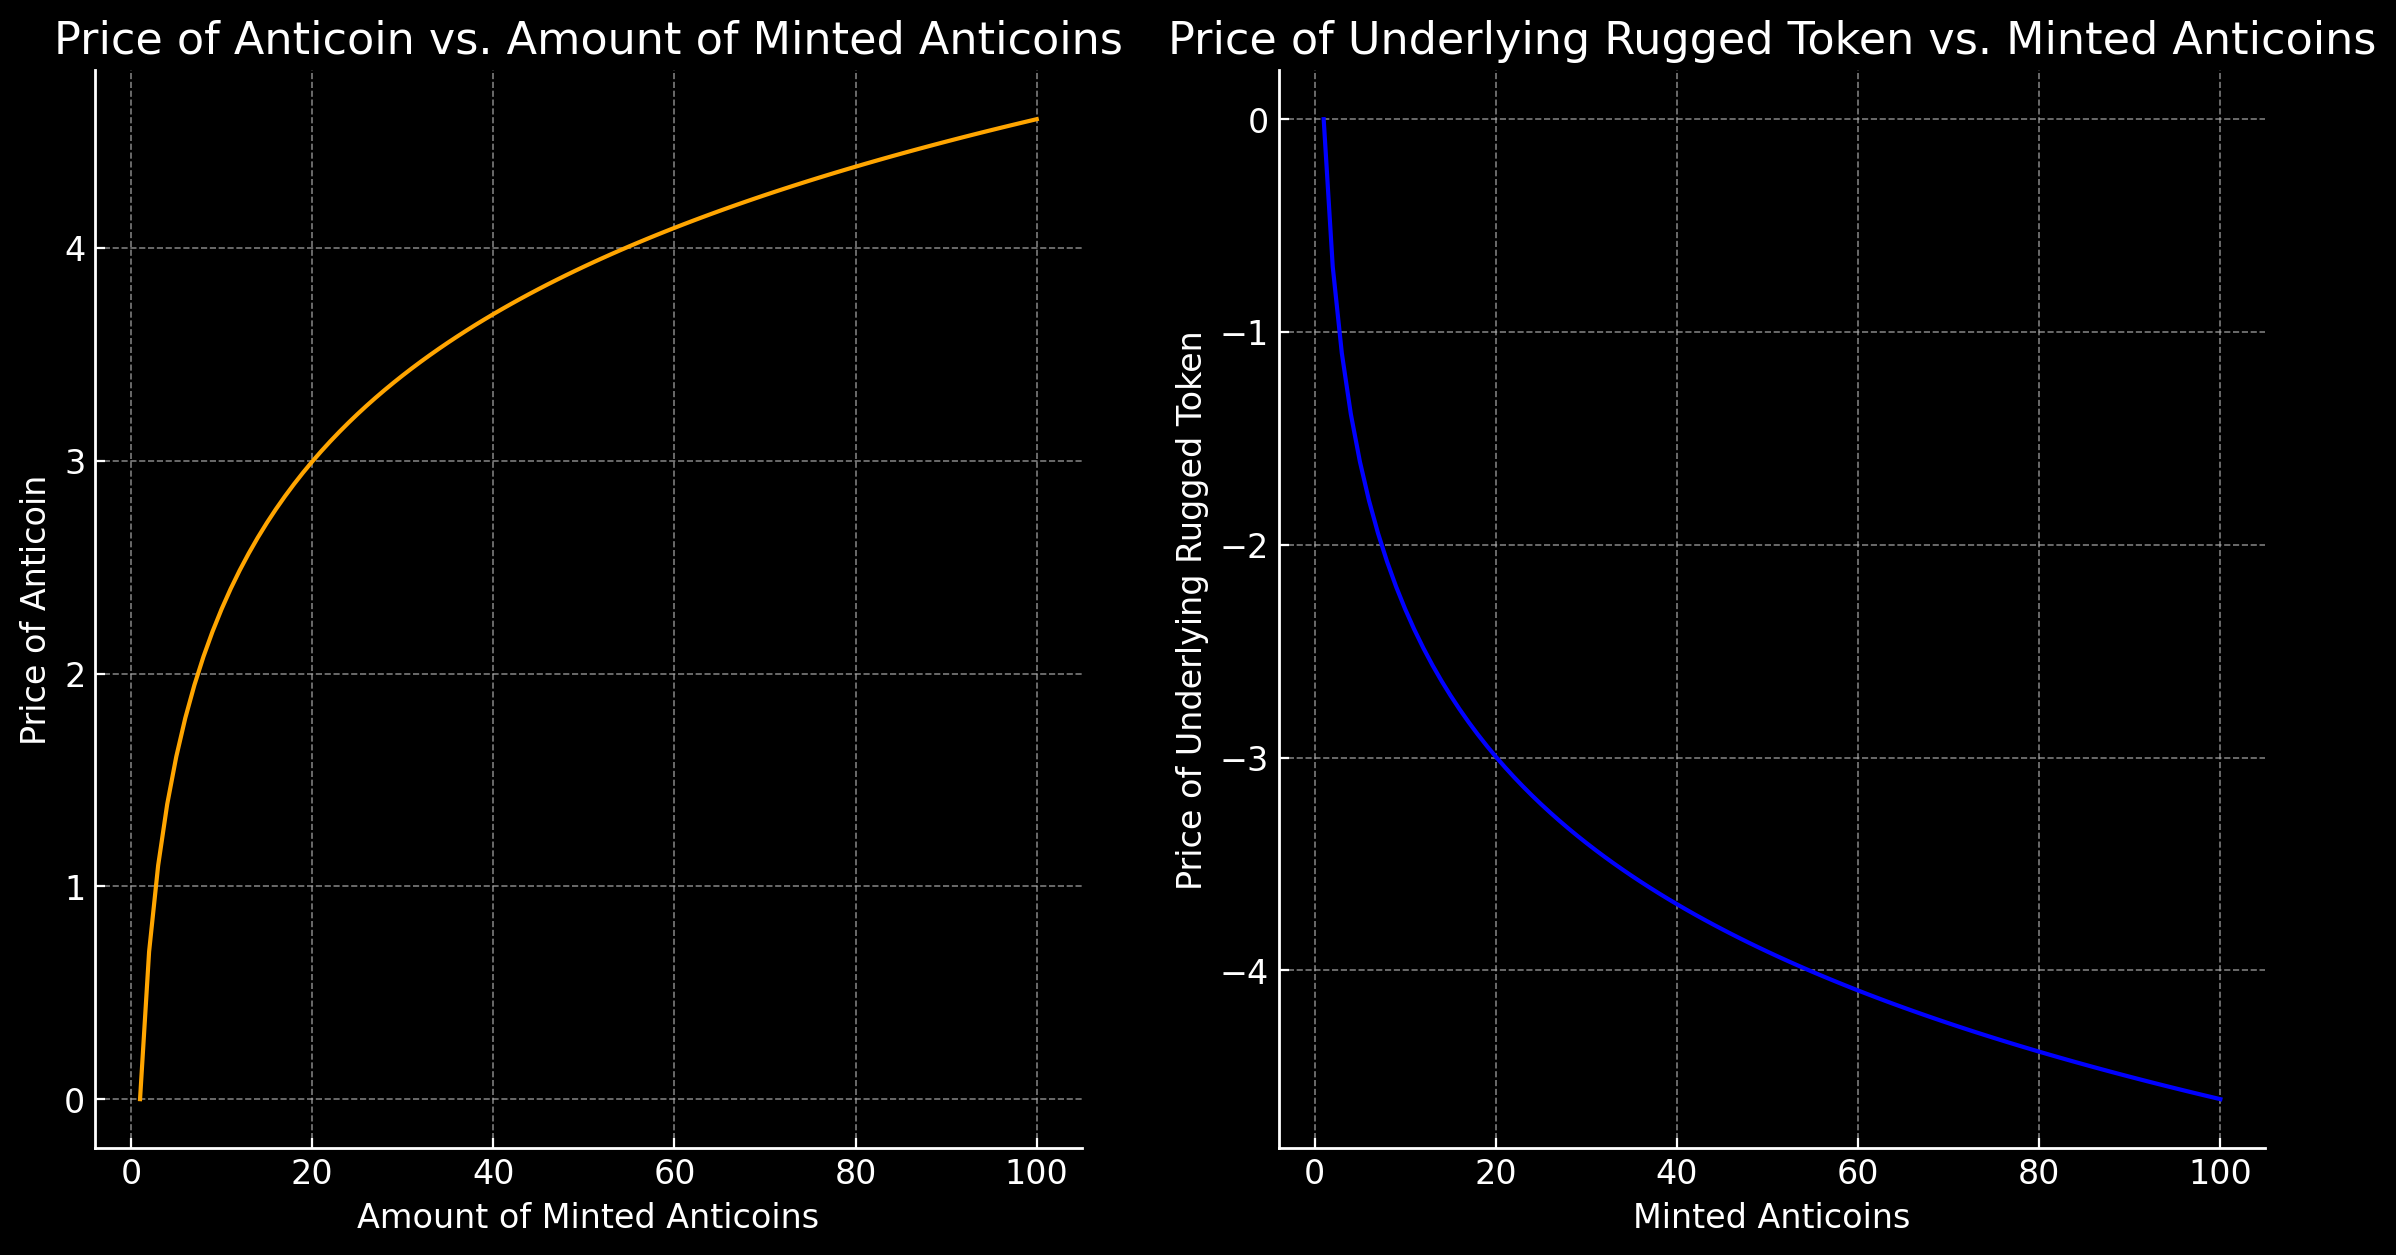
\includegraphics[width=0.8\textwidth]{images/2.png}
\caption{The inverse logarithmic relationship between the price of the underlying rugged token $C_r$ and the amount of minted anticoins $C_a$. As the price of $C_r$ decreases, the amount of minted $C_a$ increases, providing stability and protection for holders.}
\label{fig:minted_anticoins}
\end{figure}

\subsection{User Commitment and Signal to the Ecosystem}
Depositing $C_r$ into a vault $V_c$ and receiving $C_a$ signals the user's belief that $C_r$ is a rugged token. To further reinforce this belief, users can burn their $C_a$ tokens, effectively removing them from circulation and indicating their strong commitment to the protocol's mission.

\begin{equation}
\text{Signal} = \text{Burn}(C_a)
\end{equation}

This burning mechanism not only signals the user's conviction but also impacts the market by reducing the circulating supply of $C_a$. As $C_a$ tokens are burned, the inverse relationship between the price of $C_a$ and $C_r$ continues to hold, but with a nuanced adjustment reflecting the decreased supply of $C_a$.

\begin{figure}[h]
\centering
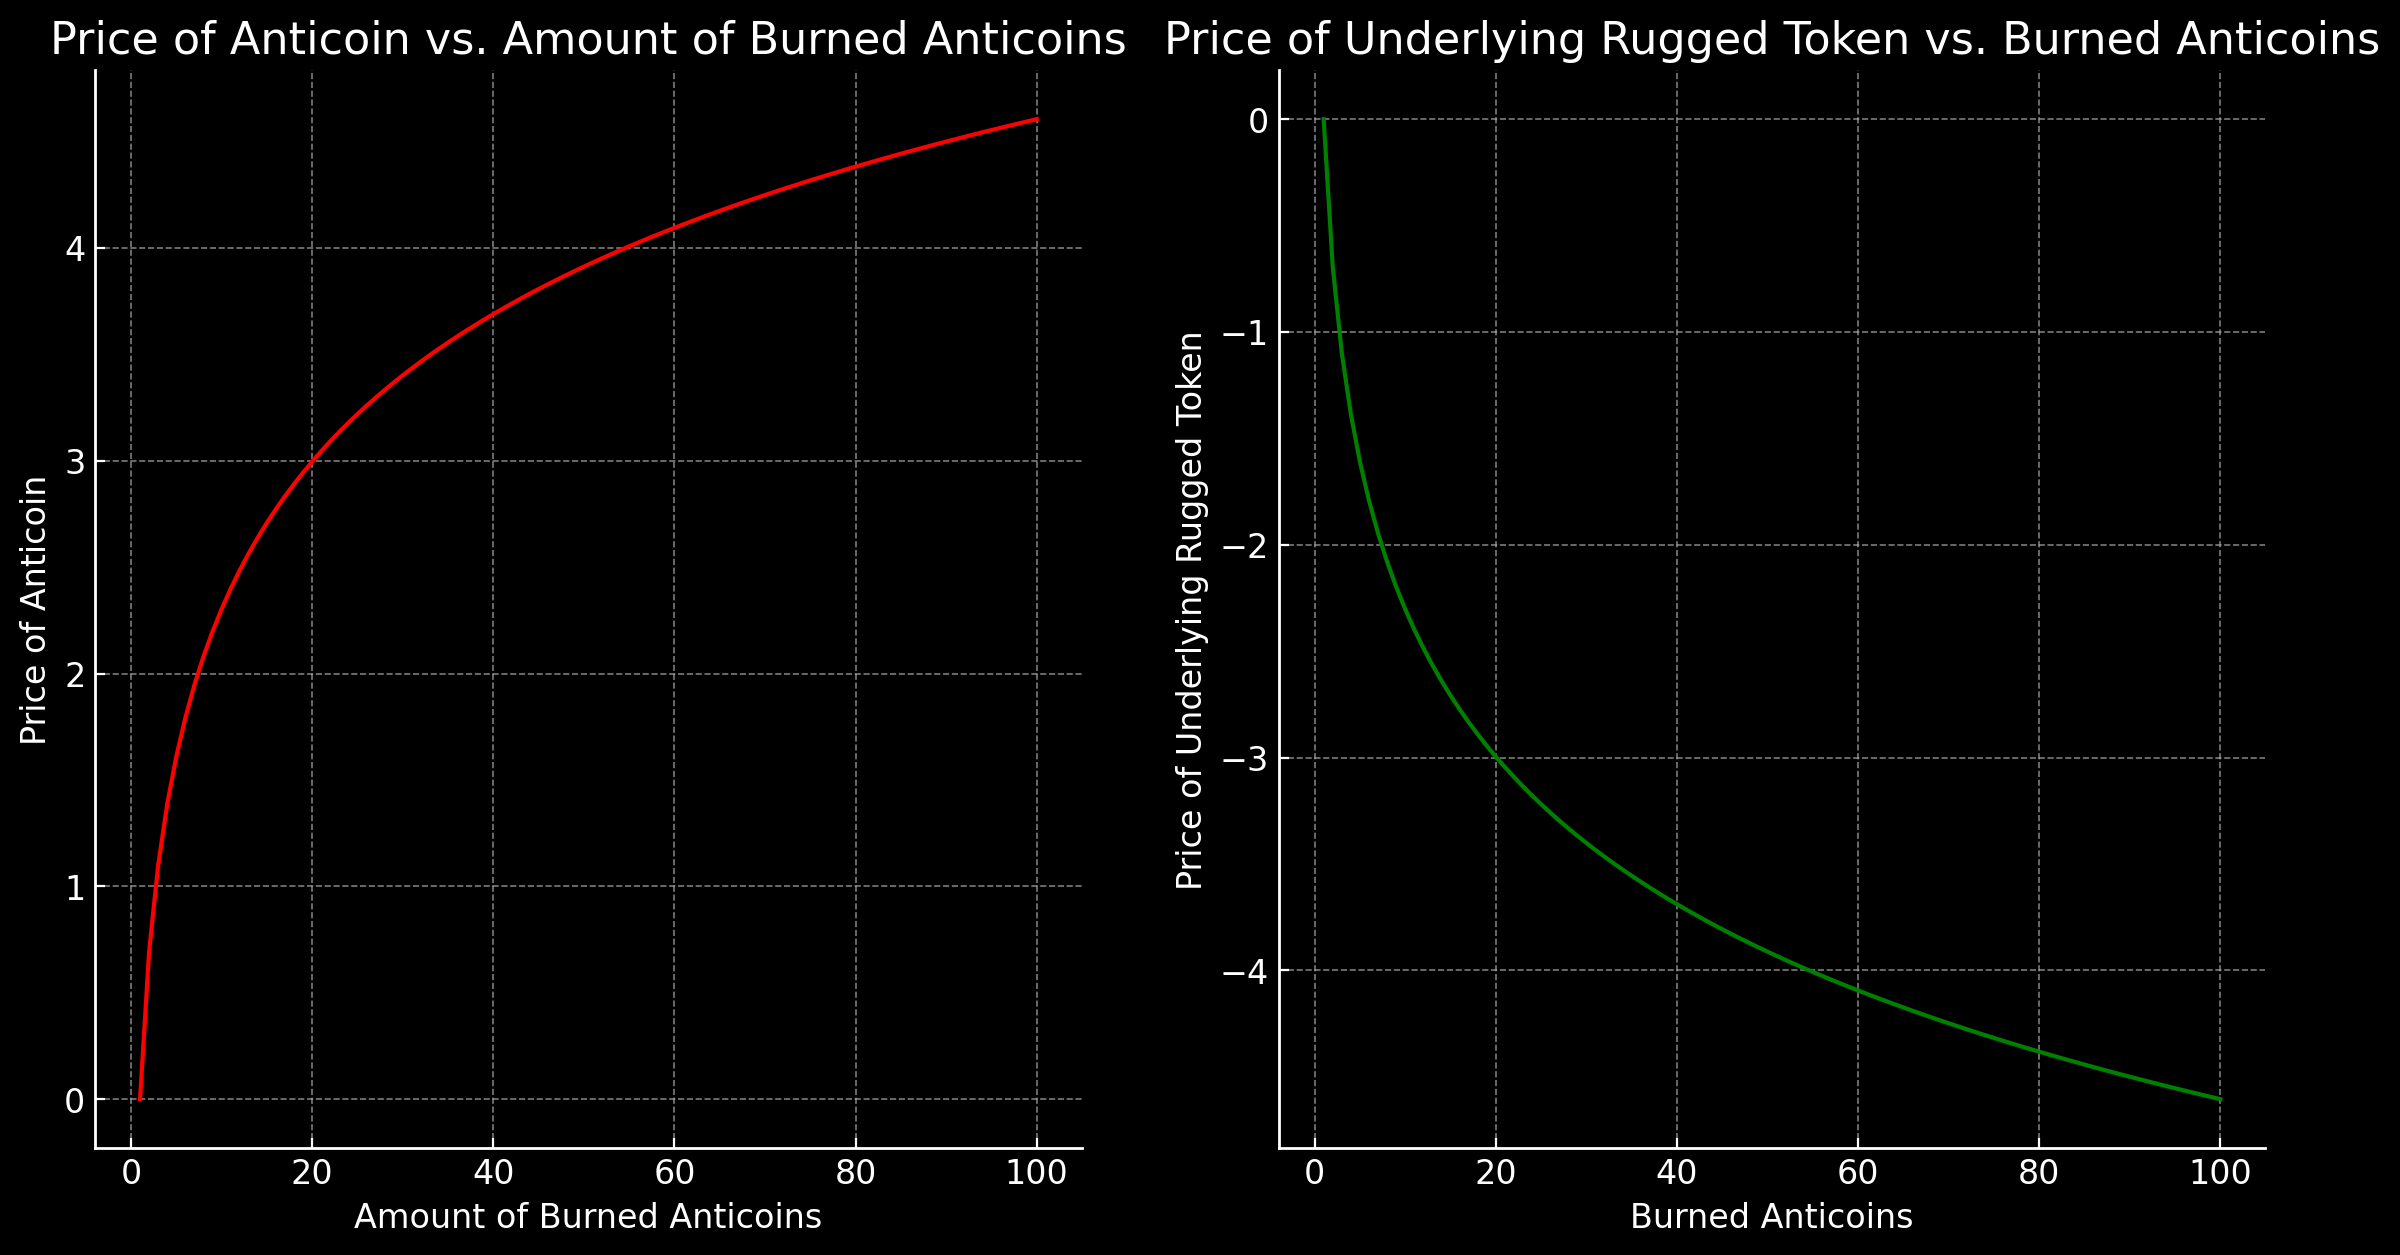
\includegraphics[width=0.8\textwidth]{images/3.png}
\caption{The adjusted inverse logarithmic relationship between the price of the underlying rugged token $C_r$ and the amount of burned anticoins $C_a$. As the price of $C_r$ decreases, the amount of burned $C_a$ decreases, further solidifying the protective mechanism for holders.}
\label{fig:burned_anticoins}
\end{figure}


%%%%%%%%%%%%%%%%%%%%%%%




\subsection{Opportunities for New Ecosystems}
The Rugsafe protocol's structure opens up opportunities for developers to build applications that cater to the needs of rug pull victims. By establishing a market for anticoin tokens $C_a$, new financial products and services can be developed to support users who have suffered losses from rug pulls. 













%%%%%%%%%%%%%%%%%%%%%%%%


\subsection{Whale Penalty Mechanism}
To prevent large holders (whales) from gaming the system, the penalty for withdrawing $C_r$ scales with the amount of $C_a$ held. Inspired by quadratic voting schemes, the penalty increases progressively as the whale's holdings increase, ensuring fairness and preventing manipulation.

\begin{equation}
P(C_a) \propto \left(\text{Holdings}\right)^\lambda
\end{equation}

Where $\lambda > 1$ is a scaling factor that ensures the penalty increases non-linearly with the amount of $C_a$ held. This scaling penalty ensures that the system remains equitable and prevents disproportionate influence by large holders.

\section{Closing Remarks}
Rugsafe presents a robust mathematical framework designed to protect against rug pulls in the DeFi space. By combining vault mechanisms, anticoin issuance, and incentive structures, it ensures a secure environment for digital asset management. The protocol's design not only protects users but also opens up new avenues for development and innovation in the DeFi ecosystem.

\end{document}
